\documentclass[aspectratio=169, 10pt]{beamer}
\usetheme{metropolis}
\metroset{block=fill, progressbar=frametitle, numbering=fraction}

\usepackage{amsmath, amssymb}
\usepackage{bm}
\usepackage{booktabs}
\usepackage{graphicx}
\usepackage{xcolor}
\usepackage{tikz}
\usetikzlibrary{arrows.meta, positioning}
\setlength{\leftmargini}{1.5em}

% Custom colors
\definecolor{koop}{RGB}{0,95,160}
\definecolor{lista}{RGB}{180,40,40}
\definecolor{mlpgreen}{RGB}{50,130,50}

\setbeamertemplate{navigation symbols}{}

% ---- Title info ----
\title[Sparse Koopman Autoencoders]{Modeling Nonlinear Dynamical Systems\\[4pt]with Sparse Koopman Autoencoders}
\author{Aidan Li \and Sujin Yun}
\institute{MAT6215 -- Dynamical Systems \\ Université de Montréal}
\date{April 2026}

% ============================================================
\begin{document}
% ============================================================

\begin{frame}
  \titlepage
\end{frame}

% ----------------------------------------------------------
\begin{frame}{Outline}
  \tableofcontents
\end{frame}

% ============================================================
\section{Motivation}
% ============================================================

%% 1-a -----------------------------------------------------------
\begin{frame}{1-a. Linear vs Nonlinear Dynamical Systems}

\begin{columns}[T,onlytextwidth]

\begin{column}{0.48\textwidth}

\textbf{Linear systems}

\[
x_{k+1} = a x_k
\]

\begin{itemize}
\item Predictable behaviour
\item Rich analysis and control tools: LQR, MPC
\end{itemize}

\vspace{0.7em}

\end{column}

\begin{column}{0.48\textwidth}

\textbf{Nonlinear systems}

\[
x_{k+1} = a x_k + b x_k^2
\]

\begin{itemize}
\item More realistic; admits chaos, bifurcations, multiple fixed points 
\item Harder prediction and control
\end{itemize}

\end{column}

\end{columns}

\vspace{0.4em}
\centering


\end{frame}


%% 1-b -----------------------------------------------------------
\begin{frame}{1-b. Can We Transform Nonlinear Systems Into Linear Ones?}

Can we map the original state $x_k$ into a new representation $z_k$
so that the dynamics evolve \textbf{approximately linearly}?
\[
z_k = \varphi(x_k), \quad z_{k+1} \approx K z_k
\]


\centering
If yes, we can use \textbf{linear tools} in the lifted space.

\vspace{0.7em}

% \begin{alertblock}{Challenge}
% The lifting $\varphi$ is unknown, and linearity may only hold approximately.
% \end{alertblock}

\end{frame}


%% 1-c -----------------------------------------------------------
\begin{frame}{1-c. From Local to Basin Linearization}

\begin{block}{Local result: Hartman--Grobman}
Near a hyperbolic fixed point $x^\star$, a nonlinear system is locally
topologically conjugate to its linearization:
\[
z_{k+1} = A z_k, \qquad A = J_F(x^\star)
\]
\end{block}

\vspace{0.4em}

\begin{block}{Beyond local}
For an attracting hyperbolic fixed point, linearizing / Koopman coordinates
can extend to the \textbf{entire basin of attraction} under additional assumptions.
\end{block}

\vspace{0.4em}
\centering


\vspace{1.2em}
\footnotesize
Hartman--Grobman (local); Lan \& Mezi\'c (2013), Kvalheim \& Revzen (2021) (basin-wide).

\end{frame}



%% 1-d -----------------------------------------------------------
\begin{frame}{1-d. Koopman Operator Theory}
  \begin{columns}
    \begin{column}{0.52\textwidth}
      \textbf{Key idea} [Koopman, 1931]\\
      % \vspace{5pt}
      Instead of evolving the state $x_k$ directly, track the evolution of
      \emph{observable functions} $g : \mathbb{R}^{d_x} \to \mathbb{R}$:
      \[
        (\mathcal{K}\, g)(x) = g(F(x))
      \]
      The Koopman operator $\mathcal{K}$ is \textbf{linear} (even if $F$ is not),
      but acts on an \emph{infinite-dimensional} function space.

      \vspace{0.7em}
      \textbf{Practical approximation}\\
      Learn a finite-dimensional lifting $\varphi$, decoder $\psi$, and
      linear transition $K$ jointly:
      \[
        z_k = \varphi(x_k),\quad z_{k+1} \approx K z_k,\quad \hat{x}_{k+1} = \psi(z_{k+1})
      \]
      % \vspace{5pt}
    \end{column}
    \begin{column}{0.44\textwidth}
  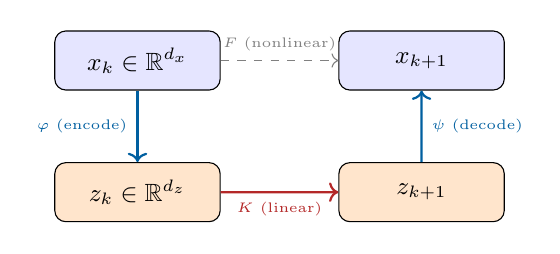
\begin{tikzpicture}[scale=0.88, every node/.style={font=\small}]
  \node[draw, rounded corners, fill=blue!10, minimum width=2.1cm, minimum height=0.75cm]
    (xk) at (0,0) {$x_k \in \mathbb{R}^{d_x}$};
  \node[draw, rounded corners, fill=orange!20, minimum width=2.1cm, minimum height=0.75cm]
    (zk) at (0,-1.9) {$z_k \in \mathbb{R}^{d_z}$};
  \node[draw, rounded corners, fill=orange!20, minimum width=2.1cm, minimum height=0.75cm]
    (zk1) at (4.1,-1.9) {$z_{k+1}$};
  \node[draw, rounded corners, fill=blue!10, minimum width=2.1cm, minimum height=0.75cm]
    (xk1) at (4.1,0) {$x_{k+1}$};

  \draw[->, thick, koop] (xk)  -- node[left]{\tiny $\varphi$ (encode)} (zk);
  \draw[->, thick, lista] (zk)  -- node[below]{\tiny $K$ (linear)} (zk1);
  \draw[->, thick, koop] (zk1) -- node[right]{\tiny $\psi$ (decode)} (xk1);
  \draw[->, dashed, gray] (xk)  -- node[above]{\tiny $F$ (nonlinear)} (xk1);
\end{tikzpicture}


      \vspace{0.4em}
      \centering\small Koopman autoencoder pipeline

      \vspace{0.5em}
      \raggedright\small
      Related work: DMD, eDMD [Schmid 2010; Williams et al.\ 2015],
      deep autoencoders [Lusch et al.\ 2018; Azencot et al.\ 2020]
    \end{column}
  \end{columns}
\end{frame}





%% 1-e -----------------------------------------------------------
\begin{frame}{1-e. Multiple Basins Break a Single Linearization}

\textbf{Key limitation}\\

Any system with multiple fixed points or any more general attractors cannot admit a single finite-dimensional Koopman-invariant subspace. 


\begin{itemize}
\item All finite-dimensional linear systems have a single fixed point
\item Cannot be topologically conjugate to a system with multiple fixed points
\item One global linear operator $K$ cannot fit them all
\end{itemize}


\vspace{1.2em}
\footnotesize
Brunton et al.\ (2016); Liu, Ozay, \& Sontag (2025).

\end{frame}

% ============================================================
\section{Approach}
% ============================================================

%% 2-a -----------------------------------------------------------
\begin{frame}{2-a. Desired Property: Basin-Support Alignment}

\begin{block}{Goal}
Learn a lifting $z = \varphi(x)$ such that
\[
z_{k+1} \approx K z_k
\]
while different basins use different sparse supports: set of indices where $z$ is non-zero.
\end{block}

\vspace{0.2em}

\textbf{One setup:}
\[
x \in \mathcal{B}_1 \mapsto z = (\star,\star,0,0), \qquad
x \in \mathcal{B}_2 \mapsto z = (0,0,\star,\star)
\]

\begin{itemize}
\item Same basin $\Rightarrow$ shared local linear coordinates
\item Different basins $\Rightarrow$ different active coordinates
\end{itemize}

\begin{exampleblock}{Desired outcome}
\vspace{0.1em}
One latent linear model can approximate different local linear regimes
through different support patterns.
\end{exampleblock}

\end{frame}



%% 2-b -----------------------------------------------------------
\begin{frame}{2-b. Why Sparsity Is a Useful Inductive Bias}

When we reconstruct $x$ using the decoder:
\[
x \approx \psi z, \qquad \|z\|_0 \ll d_z
\]

\begin{itemize}
\item Only a few latent coordinates are active for each state
\item The support $\operatorname{supp}(z)$ can act like a regime indicator
\item Different supports give a union-of-subspaces view of the state space
\end{itemize}

\vspace{0.3em}
\textbf{Sparse coding view}
\[
\min_z
\frac{1}{2}\|x - \psi z\|_2^2
+
\lambda \|z\|_1
\]

\begin{itemize}
\item Reconstruction term encourages accurate representation
\item $\ell_1$ penalty enforces sparsity
\end{itemize}

% \vspace{0.4em}

\vspace{0.2em}
Each \textbf{sparse support pattern} should correspond to a
\textbf{locally linear dynamical regime}.

\end{frame}


%% 2-c -----------------------------------------------------------
\begin{frame}{2-c. Sparse Koopman Autoencoder}

\textbf{Use a sparse encoder inside a Koopman autoencoder}

\begin{center}
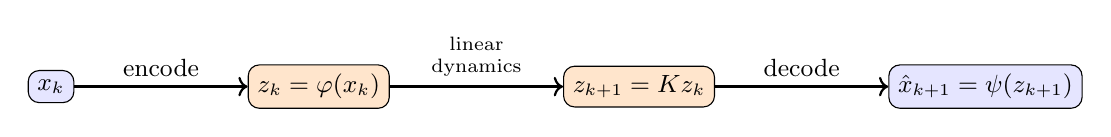
\begin{tikzpicture}[node distance=2.2cm, every node/.style={font=\small}]
\node[draw, rounded corners, fill=blue!10] (xk) {$x_k$};
\node[draw, rounded corners, fill=orange!20, right=of xk] (zk) {$z_k = \varphi(x_k)$};
\node[draw, rounded corners, fill=orange!20, right=of zk] (zk1) {$z_{k+1} = K z_k$};
\node[draw, rounded corners, fill=blue!10, right=of zk1] (xk1) {$\hat{x}_{k+1} = \psi(z_{k+1})$};

\draw[->, thick] (xk) -- node[above]{encode} (zk);
\draw[->, thick] (zk) -- node[above, align=center, font=\scriptsize]{linear\\dynamics} (zk1);
\draw[->, thick] (zk1) -- node[above]{decode} (xk1);
\end{tikzpicture}
\end{center}

\begin{itemize}
\item Replace the dense encoder with a \textbf{LISTA-style sparse encoder} meant for \textit{sparse coding}
\item Learn sparse latent coordinates, linear $K$, and decoder jointly
\item During long rollouts, periodically decode and re-encode the latent $z$ every $m$ steps to correct latent representation drift and allow for identification of the appropriate locally linear regime \[
z_{k+m} = \varphi(\psi(K^m z_k))
\]
\end{itemize}

\end{frame}


% ============================================================
\section{Experiments \& Results}
% ============================================================
\begin{frame}{Experimental Setup}

\begin{columns}

\begin{column}{0.48\textwidth}

\textbf{Benchmark: Dysts} (Gilpin 2021, 2023)

\begin{itemize}
\item 15 chaotic dynamical systems
\item Mostly $d_x = 3$ (one $d_x = 6$ system)
\item Selected for \textbf{multi-basin behaviour}
\end{itemize}

\vspace{0.5em}

Examples:
\begin{itemize}
\item Duffing oscillator
\item MultiChua
\item Shimizu–Morioka
\item Coupled Lorenz
\end{itemize}

\end{column}

\begin{column}{0.48\textwidth}

\textbf{Training setup}

\begin{itemize}
\item 200 trajectories per split
\item 30k states per trajectory
\item 10 random seeds per system
\end{itemize}

\vspace{0.5em}

\textbf{Evaluation}

\begin{itemize}
\item Long-horizon forecasting
\item Horizons: $H = 1000, 3000$
\item Metric: \textbf{MSE (IQM across seeds)}
\end{itemize}

\end{column}

\end{columns}

\vspace{0.5em}

% \begin{alertblock}{Important}
% No basin labels or regime annotations are used.
% \end{alertblock}

\end{frame}

\begin{frame}{Main Result}

\vspace{0.5em}
\textbf{Long-horizon forecasting on Dysts benchmark}

\vspace{0.5em}

\begin{center}

\begin{tabular}{lccc}
\toprule
Model & Wins (H=1000) & Wins (H=3000) & Median Error (H=3000) \\
\midrule
MLP & 2/15 & 0/15 & $1.39 \times 10^{-1}$ \\
MLP + $\ell_1$ & 1/15 & 2/15 & $7.74 \times 10^{-2}$ \\
\textbf{LISTA (ours)} & \textbf{12/15} & \textbf{13/15} & \textbf{$4.72 \times 10^{-2}$} \\
\bottomrule
\end{tabular}

\end{center}

\vspace{0.5em}

\begin{exampleblock}{Key Result}
\vspace{5pt}
LISTA achieves the best forecasting accuracy on the majority of systems. Adding an $\ell_1$ penalty helps, but the explicit sparse-coding encoder helps more.

\end{exampleblock}

\end{frame}


\begin{frame}{3000-Step Forecast Examples}

\textbf{Phase portraits in the $(x_1, x_2)$ plane for two Dysts systems}

\begin{center}
    
\includegraphics[width=0.96\textwidth]{figures/dysts_duffing_lorenzcoupled_h3000_forecasts.png}
\end{center}

\begin{exampleblock}{Qualitative read}
\vspace{5pt}
The same sparse-coding Koopman approach can handle both a lower-dimensional Duffing system
and the higher-dimensional LorenzCoupled system.
\end{exampleblock}

\end{frame}


\begin{frame}{20000-Step Forecast Examples}

\begin{center}
    
\includegraphics[width=\textwidth]{figures/dysts_dadras_qichen_shimizumorioka_h20000_subfigures.png}
\end{center}

\end{frame}


\begin{frame}{Takeaways}
  \begin{itemize}
    \item Multi-basin systems are a natural obstacle for a single global linear latent model.
    \item Koopman theory gives the linear-latent viewpoint, periodic re-encoding refreshes local coordinates, and sparse coding provides a candidate regime variable through latent support.
    \item The LISTA-based sparse-coding Koopman model improves long-horizon forecasting on most benchmark systems.
  \end{itemize}

  \vfill
  \centering
  \Large \textbf{Questions?}

\end{frame}
% ----------------------------------------------------------
\begin{frame}{References}
  \tiny
  \begin{itemize}
    \item Koopman, B.O. (1931). Hamiltonian Systems and Transformation in Hilbert Space. \textit{PNAS}.
    \item Lan \& Mezi\'c (2013). Linearization in the large of nonlinear systems. \textit{Physica D}.
    \item Brunton et al. (2016). Koopman Invariant Subspaces\ldots \textit{PLOS ONE}.
    \item Brunton et al. (2022). Modern Koopman Theory for Dynamical Systems. \textit{SIAM Review}.
    \item Schmid, P.J. (2010). Dynamic mode decomposition. \textit{J. Fluid Mech.}
    \item Williams et al. (2015). A Data-Driven Approximation of the Koopman Operator. \textit{J. Nonlinear Sci.}
    \item Lusch et al. (2018). Deep learning for universal linear embeddings. \textit{Nature Commun.}
    \item Azencot et al. (2020). Forecasting Sequential Data Using Consistent Koopman Autoencoders. \textit{ICML}.
    \item Fathi et al. (2023). Course Correcting Koopman Representations. \textit{ICLR 2024}.
    \item Olshausen \& Field (1996). Emergence of simple-cell receptive field properties. \textit{Nature}.
    \item Gregor \& LeCun (2010). Learning Fast Approximations of Sparse Coding. \textit{ICML}.
    \item Gilpin, W. (2021). Chaos as an interpretable benchmark. \textit{NeurIPS}.
    \item Gilpin, W. (2023). Model scale versus domain knowledge. \textit{Phys. Rev. Research}.
    \item Korda \& Mezi\'c (2018). Linear predictors for nonlinear dynamical systems. \textit{Automatica}.
  \end{itemize}
\end{frame}

\end{document}
